\documentclass[11pt,a4paper]{article}
\usepackage{kotex}
\setmainhangulfont[AutoFakeBold=2,AutoFakeSlant=.2]{Noto Serif CJK KR}
\setsanshangulfont[AutoFakeBold=2,AutoFakeSlant=.2]{Noto Sans CJK KR}
\usepackage[margin=25mm]{geometry}
\usepackage{amsmath,amssymb,mathtools}
\usepackage{graphicx,booktabs,array,float,xcolor,xurl,enumitem}
\usepackage{hyperref}
\usepackage[nameinlink,noabbrev]{cleveref}
\definecolor{navy}{HTML}{17324D}
\definecolor{teal}{HTML}{147D92}
\definecolor{orange}{HTML}{D97720}
\hypersetup{colorlinks=true,linkcolor=navy,citecolor=teal,urlcolor=orange}
\setlist{nosep,leftmargin=*}
\newcommand{\mpl}{M_{\mathrm{Pl}}}
\newcommand{\eps}{\epsilon_{\mathrm{th}}}
\newcommand{\qnum}{Q_{\mathrm{num}}}
\newcommand{\qlr}{Q_{\mathrm{LR}}}
\newcommand{\qsurf}{Q_{\mathrm{surf}}}
\newcommand{\qctr}{Q_{\mathrm{ctr}}}
\newcommand{\qms}{Q_{\mathrm{MS}}}
\newcommand{\qpv}{Q_{\mathrm{PV}}}
\newcommand{\qas}{Q_{\mathrm{AS}}}
\newcommand{\ad}{\alpha_{\mathrm{direct}}}
\newcommand{\at}{\alpha_{\mathrm{tail}}}
% Generated by run_study.py; do not edit individual numbers.
\newcommand{\StudyPoints}{725}
\newcommand{\StudySurfaceWithin}{68.8}
\newcommand{\StudyCenterWithin}{91.3}
\newcommand{\StudyASWithin}{99.7}
\newcommand{\StudyASMedian}{0.391}
\newcommand{\StudyASMax}{13.1}
\newcommand{\StudyASLocalMax}{22.9}
\newcommand{\StudyASLocalWithin}{85.2}
\newcommand{\StudyPointMedian}{0.378}
\newcommand{\StudyPointMax}{12.7}
\newcommand{\StudyRadialMax}{1.51}
\newcommand{\StudyForceNearMax}{16.6}
\newcommand{\StudyForceNearFailures}{100}
\newcommand{\StudyForceFiveMax}{3.85}
\newcommand{\StudyForceTenMax}{1.84}
\newcommand{\StudyValidityRadiusMax}{2.25}
\newcommand{\StudyRadiusSamples}{71}
\newcommand{\StudyTailFlips}{2}
\newcommand{\StudySurfaceFlips}{1}
\newcommand{\StudyCenterFlips}{3}
\newcommand{\StudyAnsatzDisagreement}{4}
\newcommand{\StudyBothWrong}{0}
\newcommand{\StudyAuditPoints}{16}
\newcommand{\StudyAuditChargeMax}{0.056}
\newcommand{\StudyAuditForceMax}{0.0026}
\newcommand{\StudyAuditForceFlips}{0}
\newcommand{\StudyGatePoints}{17}
\newcommand{\StudyGateCoverage}{2.34}
\newcommand{\StudyGateHeldout}{12}
\newcommand{\StudyWeakError}{2.7\times10^{-5}}
\newcommand{\StudyThreshold}{10^{-2}}
\newcommand{\StudySurfaceShift}{0.00156}
\newcommand{\StudyCenterShift}{0.0369}

\newcommand{\StudyChargeRowsEN}{%
Surface-amplitude model & 2.78\% & 62.6\% & 499/725 \\
Center-point model & 0.566\% & 30.1\% & 662/725 \\
Finite shell volume & 2.18\% & 37.6\% & 562/725 \\
Point + finite volume & 0.378\% & 12.7\% & 723/725 \\
Active-shell integral & 0.391\% & 13.1\% & 723/725 \\
}

\newcommand{\StudyChargeRowsKO}{%
표면 진폭 모형 & 2.78\% & 62.6\% & 499/725 \\
중심점 모형 & 0.566\% & 30.1\% & 662/725 \\
유한 껍질 부피 & 2.18\% & 37.6\% & 562/725 \\
점원천+유한 부피 & 0.378\% & 12.7\% & 723/725 \\
활성 껍질 적분 & 0.391\% & 13.1\% & 723/725 \\
}

\newcommand{\StudyLocalForceRowsEN}{%
Surface-amplitude model & 1.37\% & 48.1\% & 629/725 \\
Center-point model & 0.474\% & 24\% & 594/725 \\
Finite shell volume & 0.941\% & 28.8\% & 690/725 \\
Point + finite volume & 0.423\% & 24\% & 616/725 \\
Active-shell integral & 0.424\% & 22.9\% & 618/725 \\
}

\newcommand{\StudyLocalForceRowsKO}{%
표면 진폭 모형 & 1.37\% & 48.1\% & 629/725 \\
중심점 모형 & 0.474\% & 24\% & 594/725 \\
유한 껍질 부피 & 0.941\% & 28.8\% & 690/725 \\
점원천+유한 부피 & 0.423\% & 24\% & 616/725 \\
활성 껍질 적분 & 0.424\% & 22.9\% & 618/725 \\
}

\newcommand{\StudyDistanceRows}{%
1.05 & 0.197\% & 35.4\% & 148 \\
1.5 & 0.194\% & 16.6\% & 100 \\
2 & 0.191\% & 11.6\% & 52 \\
5 & 0.165\% & 3.85\% & 0 \\
10 & 0.137\% & 1.84\% & 0 \\
}

\setlength{\emergencystretch}{2em}

\graphicspath{{figures_ko/}}
\crefname{equation}{식}{식}\Crefname{equation}{식}{식}
\crefname{figure}{그림}{그림}\Crefname{figure}{그림}{그림}
\crefname{table}{표}{표}\Crefname{table}{표}{표}
\hypersetup{pdftitle={스칼라 전하에서 국소 힘으로: 카멜레온 얇은 껍질 근사의 검증},pdfauthor={이동규}}
\title{\bfseries\Large 스칼라 전하에서 국소 힘으로\\[4pt]
\large 구대칭 카멜레온 장에서 근사 정확도,\newline 거리 의존성, 임계값 판정의 검증}
\author{이동규\\\small 서울대학교 물리천문학부\\\small 고전역학 학기말 프로젝트: 독립 개정 연구}
\date{2026년 10월 19일}

\begin{document}
\renewcommand{\abstractname}{초록}\renewcommand{\figurename}{그림}
\renewcommand{\tablename}{표}\renewcommand{\refname}{참고문헌}
\maketitle
\begin{abstract}
차폐된 원천이 만드는 제5힘을 예측할 때 원천 전체를 하나의 유효 스칼라 전하로
대체하곤 한다. 본 연구는 이 과정의 두 단계를 구분하여 검증한다. 첫째는 점근
전하의 추정이며, 둘째는 그 전하로 유한한 거리의 힘을 예측하는 것이다.
$V(\phi)=\Lambda^5/\phi$와 약한 등각 결합 극한에서 두 영역 콜로케이션 방법으로
$10^2\leq\rho_c/\rho_\infty\leq10^5$, $10^{-3}\leq m_\infty R\leq0.3$의
\StudyPoints 개 비선형 구대칭 경계값 문제를 풀었다. 활성 껍질 유카와 적분은
이 격자의 \StudyASWithin\%에서 전하를 10\% 이내로 예측한다. 그러나 점원천
인자와 유한 껍질 부피만 결합한 간단한 대조군도 같은 비율을 달성하며, 오차
중앙값은 \StudyPointMedian\%로 방사형 적분의 \StudyASMedian\%보다 조금 작다.
따라서 성능 향상을 추가적인 반지름 가중치의 효과로 확정할 수 없다. 수치적으로
정확한 점근 전하를 넣어도 $1.5R$의 국소 힘은 최대 \StudyForceNearMax\%까지
과소평가되며, \StudyForceNearFailures 개 점에서 오차가 10\%를 넘는다. 최대 오차는
$5R$에서 \StudyForceFiveMax\%, $10R$에서 \StudyForceTenMax\%로 감소한다.
예시적인 힘비 임계값 $\alpha_\star=\StudyThreshold$에서 기준값을 점근 꼬리로부터
비선형 수치 기울기로 바꾸면 \StudyTailFlips 개 판정이 달라진다. 선택한
\StudyAuditPoints 개 점의 계산 영역 및 해상도를 높여도 직접 힘의 판정은 유지된다.
이는 이상화한 모형에서 근사와 판정 경계의 유효성을 검증한 결과이며, 장치의
민감도나 새로운 실험 배제 결과를 제시하는 연구는 아니다.
\end{abstract}

\section{연구 질문과 범위}
카멜레온 차폐에서는 주변 물질의 밀도에 따라 스칼라 장이 매개하는 힘의 크기와
작용 범위가 달라진다 \cite{KhouryPRL,KhouryPRD}. 미시적인 물질 결합이 크더라도,
밀도 높은 물체의 내부 장이 거의 일정하게 유지되면 유효 스칼라 전하는 작아질
수 있다. 익숙한 장거리 얇은 껍질 근사는 이 현상을 계산 비용이 작은 하나의
수로 요약한다. 그러나 이를 관측량에 적용하는 과정에는 원천을 근사하는 단계와
그 원천이 만드는 힘을 유한한 거리까지 전파하는 단계가 모두 들어간다.

본 연구는 세 가지를 묻는다. 지정한 전하 근사식은 비선형 구대칭 해를 얼마나
정확히 재현하는가? 유한 껍질 부피 보정과 방사형 유카와 가중치는 각각 얼마나
기여하는가? 그리고 점근 전하가 국소 힘을 정확히 예측하려면 탐침이 원천에서
얼마나 떨어져야 하는가? 마지막 질문은 고전역학의 관측량과 직접 연결된다.
작은 시험 물체의 가속도를 결정하는 것은 국소 장의 기울기이기 때문이다.

유한한 내부 질량 효과를 포함하는 얇은 껍질 및 껍질 없음 정합해는 이미 연구되었고
\cite{TamakiTsujikawa}, 실제 실험실 기하에 대한 수치 계산도 존재한다
\cite{Elder2016,Schlogel2016}. 본 연구는 그 방법이나 유카와 껍질 적분의 문헌상
최초성을 주장하지 않는다. 제한된 기여는 대조군을 갖춘 전하--국소 힘 오차 분석과,
수치적 기준값을 명확히 한 임계값 판정의 재현 가능한 검증이다. 코드와 데이터는
\href{https://github.com/Lasqui-Ponto/Mechanics_Term_Project/tree/agent/improve-chameleon-project/Thin_Shell_Study}{공개 GitHub 저장소}에 있다.

\section{물리 모형과 정규화}
자연단위계 $\hbar=c=1$과 환산 플랑크 질량 $\mpl=(8\pi G)^{-1/2}$을 사용한다.
양의 스칼라 장에 대해
\begin{equation}
 V(\phi)=\frac{\Lambda^5}{\phi},\qquad A(\phi)=e^{\phi/M_c},
 \qquad M_c=\frac{\mpl}{\beta}
\end{equation}
로 두면, 정적이고 중력이 약한 영역의 방정식은
\begin{equation}
 \nabla^2\phi=-\frac{\Lambda^5}{\phi^2}+\frac{\rho}{M_c}e^{\phi/M_c}
\end{equation}
이다. 근사의 범위를 명시하기 위해 $x=r/R$, $u=\phi/\phi_\infty$,
$\widetilde\rho=\rho/\rho_\infty$, $D=\phi_\infty/M_c$를 정의한다.
완전한 무차원 방정식은
\begin{equation}
 u''+\frac2x u'=-\frac{A_0}{u^2}+B_0\widetilde\rho e^{Du},
 \quad A_0=\frac{\Lambda^5R^2}{\phi_\infty^3},\quad
 B_0=\frac{\rho_\infty R^2}{M_c\phi_\infty}
\end{equation}
이다. $\phi_\infty$를 환경의 정확한 최솟값으로 정하면 $A_0=B_0e^D$이고
$(m_\infty R)^2=A_0(2+D)$이다. 본 계산은 $D\to0$ 극한을 의도적으로 택한다.
독립적인 결합 매개변수를 무차원화 과정에서 임의로 생략한 것이 아니다.
이 극한에서는
\begin{equation}
 \phi_{\min}=\left(\frac{\Lambda^5M_c}{\rho}\right)^{1/2},\qquad
 m_{\rm eff}^2=\frac{2\Lambda^5}{\phi_{\min}^3},\qquad
 \lambda_C=m_{\rm eff}^{-1}
\end{equation}
이 된다. 두 입력을 $\delta=\rho_c/\rho_\infty$, $\mu=m_\infty R$로 정하면
\begin{equation}
 u''+\frac2x u'=\frac{\mu^2}{2}[\widetilde\rho(x)-u^{-2}],
 \quad \widetilde\rho=\begin{cases}\delta,&x<1,\\1,&x>1,\end{cases}
 \quad u'(0)=0,\quad u(\infty)=1.
 \label{eq:bvp}
\end{equation}
따라서 $u_c=\delta^{-1/2}$, $m_cR=\mu\delta^{3/4}$이다.

\subsection{얇은 껍질 매개변수와 실제 기하학적 두께의 구분}
정규화에는 물체의 총질량 $M_s=4\pi\rho_cR^3/3$과 표면 퍼텐셜
$\Phi_N=GM_s/R$을 사용하며, 다음을 정의한다.
\begin{equation}
 \eps\equiv\frac{\phi_\infty-\phi_c}{6\beta\mpl\Phi_N}
 =\frac{2(1-\delta^{-1/2})}{\mu^2\delta}.
 \label{eq:eps}
\end{equation}
이는 퍼텐셜 차이로 정의한 얇은 껍질 매개변수이며, 실제 기하학적 두께와 정확히
같은 양은 아니다. 관련된 큰 내부 질량의 점근 영역에서는
$\eps\simeq\Delta R/R+1/(m_cR)$ 같은 보정이 나타나므로, $\Delta R/R$과
동일시하려면 그 보정이 충분히 작아야 한다 \cite{TamakiTsujikawa}.
예를 들어 $(\delta,\mu)=(10^5,0.1)$에서는 $\eps=1.99\times10^{-3}$인 반면
$1/(m_cR)=1.78\times10^{-3}$이다. 이 연구에서는 가정한 껍질 반지름을 BVP에서
측정한 실제 두께라고 해석하지 않는다.

\section{전하 근사식과 성능 원인을 분리하는 대조군}
아래의 전하 예측은 모두 동일한 표면 기준 꼬리 정규화를 사용한다.
상한을 둔 장거리 선도 근사는
\begin{equation}
 \qlr=\min(3\eps,1),\qquad \mu\ll1
\end{equation}
이다. 1에서 절단하는 과정부터 전이 영역에 적용하기 위한 보간이며, 그 영역에서
오차가 통제된 전개는 아니다. 두 유한 범위 진폭 가설을
\begin{equation}
 \qsurf=\qlr,\qquad \qctr=e^{-\mu}\qlr
\end{equation}
로 정한다. 이들은 같은 계수에 대한 서로 다른 근사이며, 이론 자체의 물리적
모호성을 뜻하지 않는다. 하나의 고정된 해를 $e^{-\mu(x-1)}/x$ 대신
$e^{-\mu x}/x$로 표현하면 계수도
$Q^{\text{중심 기준}}=e^\mu Q^{\text{표면 기준}}$로 변환되고 장과 힘은 변하지
않는다. 또한 ``표면 진폭''은 실제 구면 껍질 물질이 만드는 정확한 장을 뜻하지
않는다. 유한 질량을 고려한 문헌의 정합법은 이 두 단순 가설보다 상세한 근사를
제공한다 \cite{TamakiTsujikawa}.

내부 장이 고정된 중심부와 질량 없는 외부를 정합한 모형에서는 가정한 중심부의
반지름 비 $q=\sqrt{\max(1-2\eps,0)}$와 활성 껍질 부피
\begin{equation}
 \qms=1-q^3
\end{equation}
을 얻는다. 이는 근사적 구성으로, 유한한 $\mu$에서 중심부 반지름을 자기일관되게
다시 정합한 결과는 아니다. 추가적인 반지름 가중치만 비교하기 위해
\begin{align}
 \qpv&=e^{-\mu}(1-q^3),\\
 \qas&=\frac{3e^{-\mu}}{\mu^3}[g(\mu)-g(\mu q)],
 \qquad g(z)=z\cosh z-\sinh z
 \label{eq:ablation}
\end{align}
를 비교한다. 두 식은 같은 활성 부피와 점원천 유카와 인자를 가지며, $\qas$에만
추가 구대칭 반지름 가중치가 들어간다. 전체 원천이 활성화된 선형 균일 구의
정확한 해에는 배경을 빼는 인자 $1-\delta^{-1}$도 있다.
\begin{equation}
 Q_{\rm lin}=(1-\delta^{-1})\frac{3e^{-\mu}}{\mu^3}g(\mu).
\end{equation}
껍질 모형은 고밀도 대비 격자에서 작은 이 배경 항을 생략하지만, 약한 원천의
검증에서는 이 항을 유지한다.

\section{점근 스칼라 전하와 국소 가속도}
선형화가 유효한 외부 영역에서 수치적 전하를
\begin{equation}
 u=1-s\qnum\frac{e^{-\mu(x-1)}}x,\qquad s=\frac{\mu^2\delta}{6}
\end{equation}
으로 정의한다. 적절한 꼬리 구간에서만 사용하는 두 추정량은
\begin{equation}
 Q_A=\frac{x(1-u)e^{\mu(x-1)}}s,\qquad
 Q_\nabla=\frac{x^2u'e^{\mu(x-1)}}{s(1+\mu x)}
\end{equation}
이다. 보고하는 $\qnum$은 외부의 정확한 원천항과 선형화의 차이가 2\% 미만인
구간에서 $Q_A$의 중앙값이다. $Q_\nabla$와의 일치는 꼬리 추출의 진단 기준이며,
원천 가까이에서도 선형화가 성립한다는 증거는 아니다.

원천에 미치는 되먹임을 무시할 수 있는 작은 탐침의 반응 인자를 $Q_t$라고 하자.
직접적인 비선형 기준값과 유카와 꼬리 예측은 각각
\begin{align}
 \ad(x)&=\left|\frac{a_5}{a_N}\right|_{\text{직접}}
     =\frac{2\beta^2Q_t}{s}x^2u'_{\rm num}(x),\label{eq:direct}\\
 \at(Q,x)&=2\beta^2Q_tQ(1+\mu x)e^{-\mu(x-1)}
 \label{eq:tail}
\end{align}
이다. 여기서 $a_N=GM_s/(R^2x^2)$는 원천 물체 자체의 뉴턴 가속도 기준이며,
무한한 균일 환경 전체의 가속도가 아니다. 주요 힘 계산에서는 $\beta=Q_t=1$이다.
$Q_t$는 외부에서 지정하는 반응 인자로, 두 물체의 차폐 문제를 수치적으로 푼 값은 아니다.

두 단계의 오차는 다음과 같이 곱해진다.
\begin{equation}
 \frac{\at(Q_j,x)}{\ad(x)}=
 \frac{Q_j}{\qnum}\,\frac{\at(\qnum,x)}{\ad(x)}.
 \label{eq:factorization}
\end{equation}
그러므로 전하 오차와 전파 오차는 서로 증폭되거나 상쇄될 수 있다. 전하 정확도의
순위가 국소 힘 정확도의 순위와 같다고 보장할 수 없다.

\section{수치 방법과 검증}
$x=1$의 밀도 불연속을 보존하기 위해 내부와 외부를 별도 콜로케이션 영역으로
나누어 공통 좌표에 사상한다. 표면에서 $u$와 $u'$를 정합하며, 유한 외부 경계에는
점근 로빈 조건 $u'(x_{\max})=(\mu+1/x_{\max})[1-u(x_{\max})]$을 적용한다.
조건수를 개선하기 위해 전하로 스케일한 변수 $x(u-1)=sv$를 사용하고, 양의 장
표현이 유리할 때는 $u=\exp(sv/x)$를 사용한다. 두 표현은 같은 비선형 방정식을
풀며, 얇은 껍질 해를 BVP의 정답으로 입력하지 않는다.
로빈 조건은 점근 조건이다. 로그 표현에서는 $x\log u/s$에 같은 선형 꼬리
차수로 적용하며, 남은 비선형 경계항의 영향은 계산 영역을 늘려 검사한다.

SciPy의 4차 콜로케이션 알고리즘으로 초록의 범위에 놓인 $25\times29$개 로그
격자를 푼다. 명목 계산 영역은 $x_{\max}=160$, 허용오차는 $2\times10^{-4}$이며
모든 점이 수렴했다. 각 해에서 $1.02\leq x\leq20$의 \StudyRadiusSamples 개 탐침
거리를 직접 평가하며, $1.05,1.5,2,3,5,10$을 포함한다. 약한 원천에서 알려진
균일 구의 해석적 전하를 재현하는 최대 상대오차는 $\StudyWeakError$이다.

\begin{figure}[H]\centering
 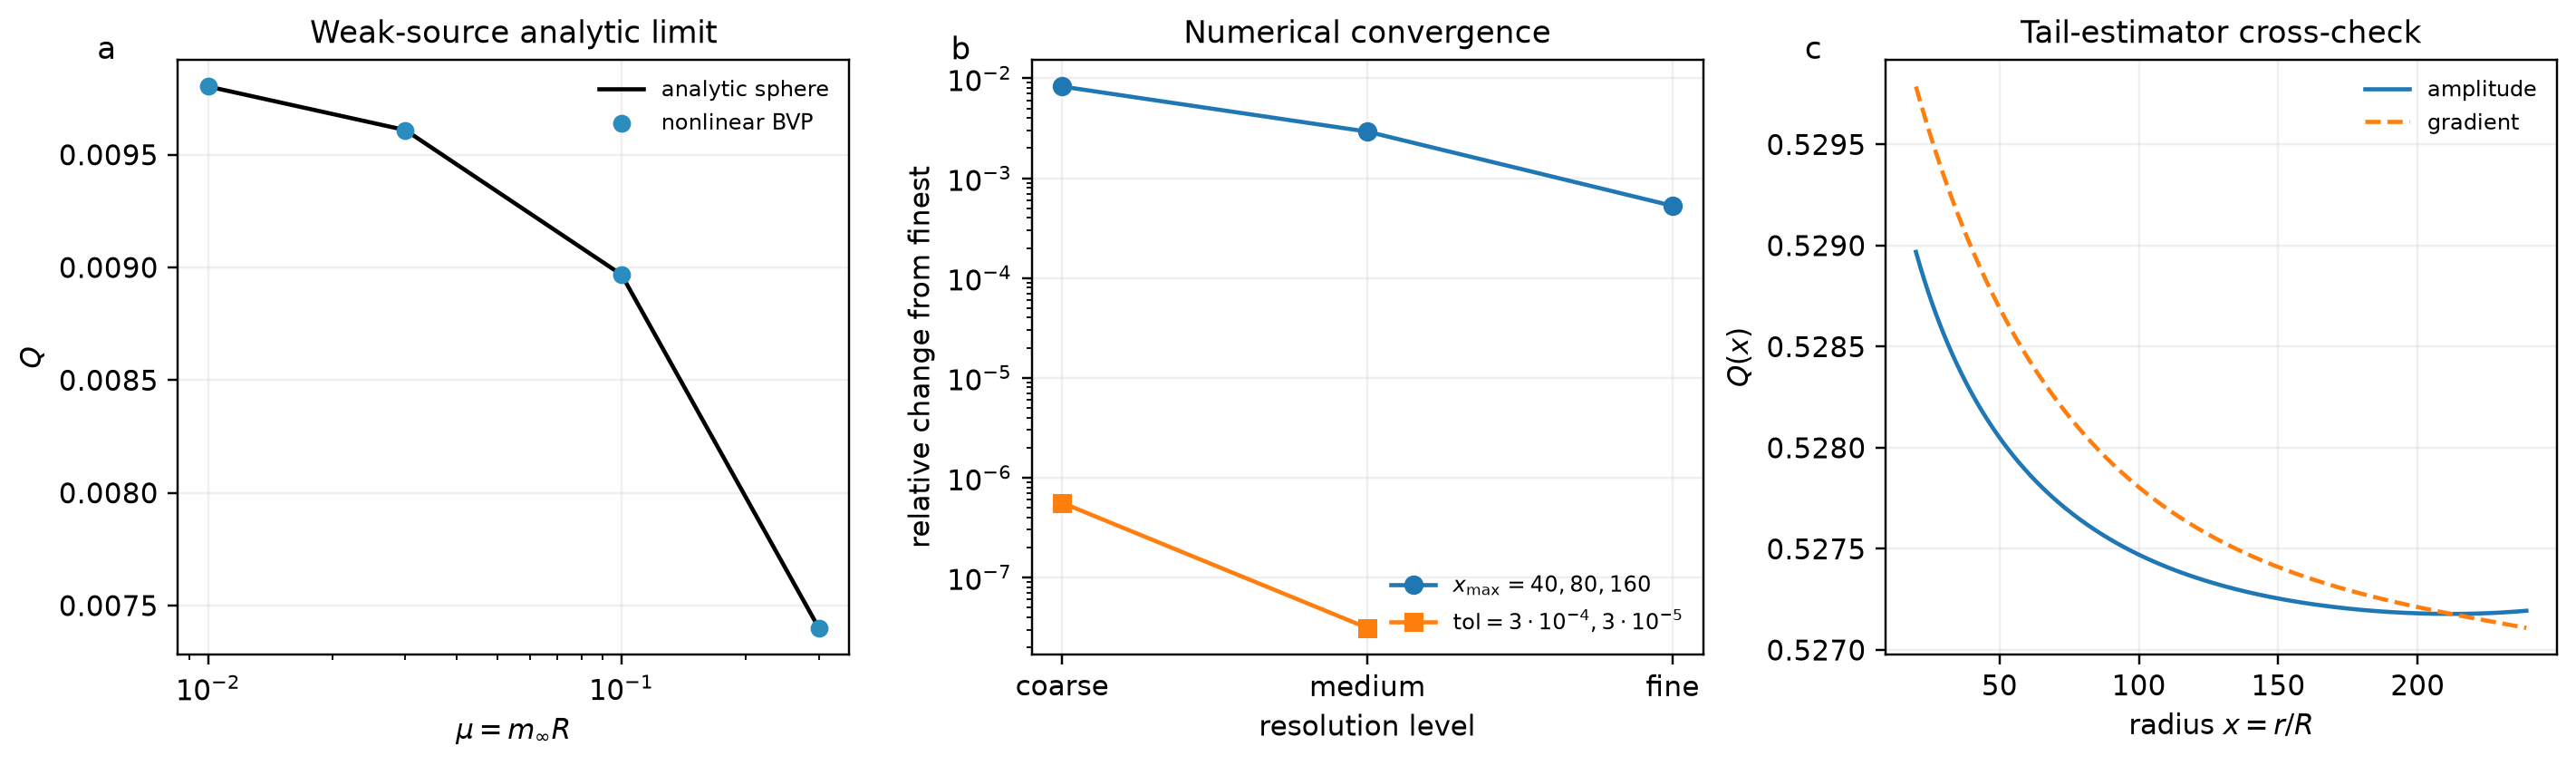
\includegraphics[width=\textwidth]{verification.png}
 \caption{해석적 극한, 해상도 수렴, 꼬리 추정량 교차검사. 두 꼬리 추정량은 하나의
 BVP 해에 대한 진단이며, 서로 독립적인 두 장 풀이 알고리즘을 뜻하지 않는다.}
\end{figure}

격자의 모서리, 대표점, 전하 근사의 10\% 오차 경계 인근, 꼬리와 직접 힘의
임계값 판정이 바뀐 점, 국소 힘 오차가 가장 큰 점을 추가 검증 대상으로 정한다.
선택된 \StudyAuditPoints 개 점에서 허용오차를 줄이고 $160R$과 $240R$을 비교했다.
전하 변화의 최댓값은 \StudyAuditChargeMax\%이며, 모든 표본 탐침 거리에서 명목
격자 계산과 정밀 계산의 국소 힘 차이는 최대 \StudyAuditForceMax\%이다.
직접 힘의 임계값 판정은 \StudyAuditForceFlips 개 점에서 바뀌었다. 이는 보고하는
차이를 뒷받침하지만 전체 격자 각각의 수렴 증명이나 연속 매개변수 영역의 오차
한계는 아니다.

\section{결과}
\subsection{전하 정확도와 대조군이 보여 주는 것}
\begin{figure}[H]\centering
 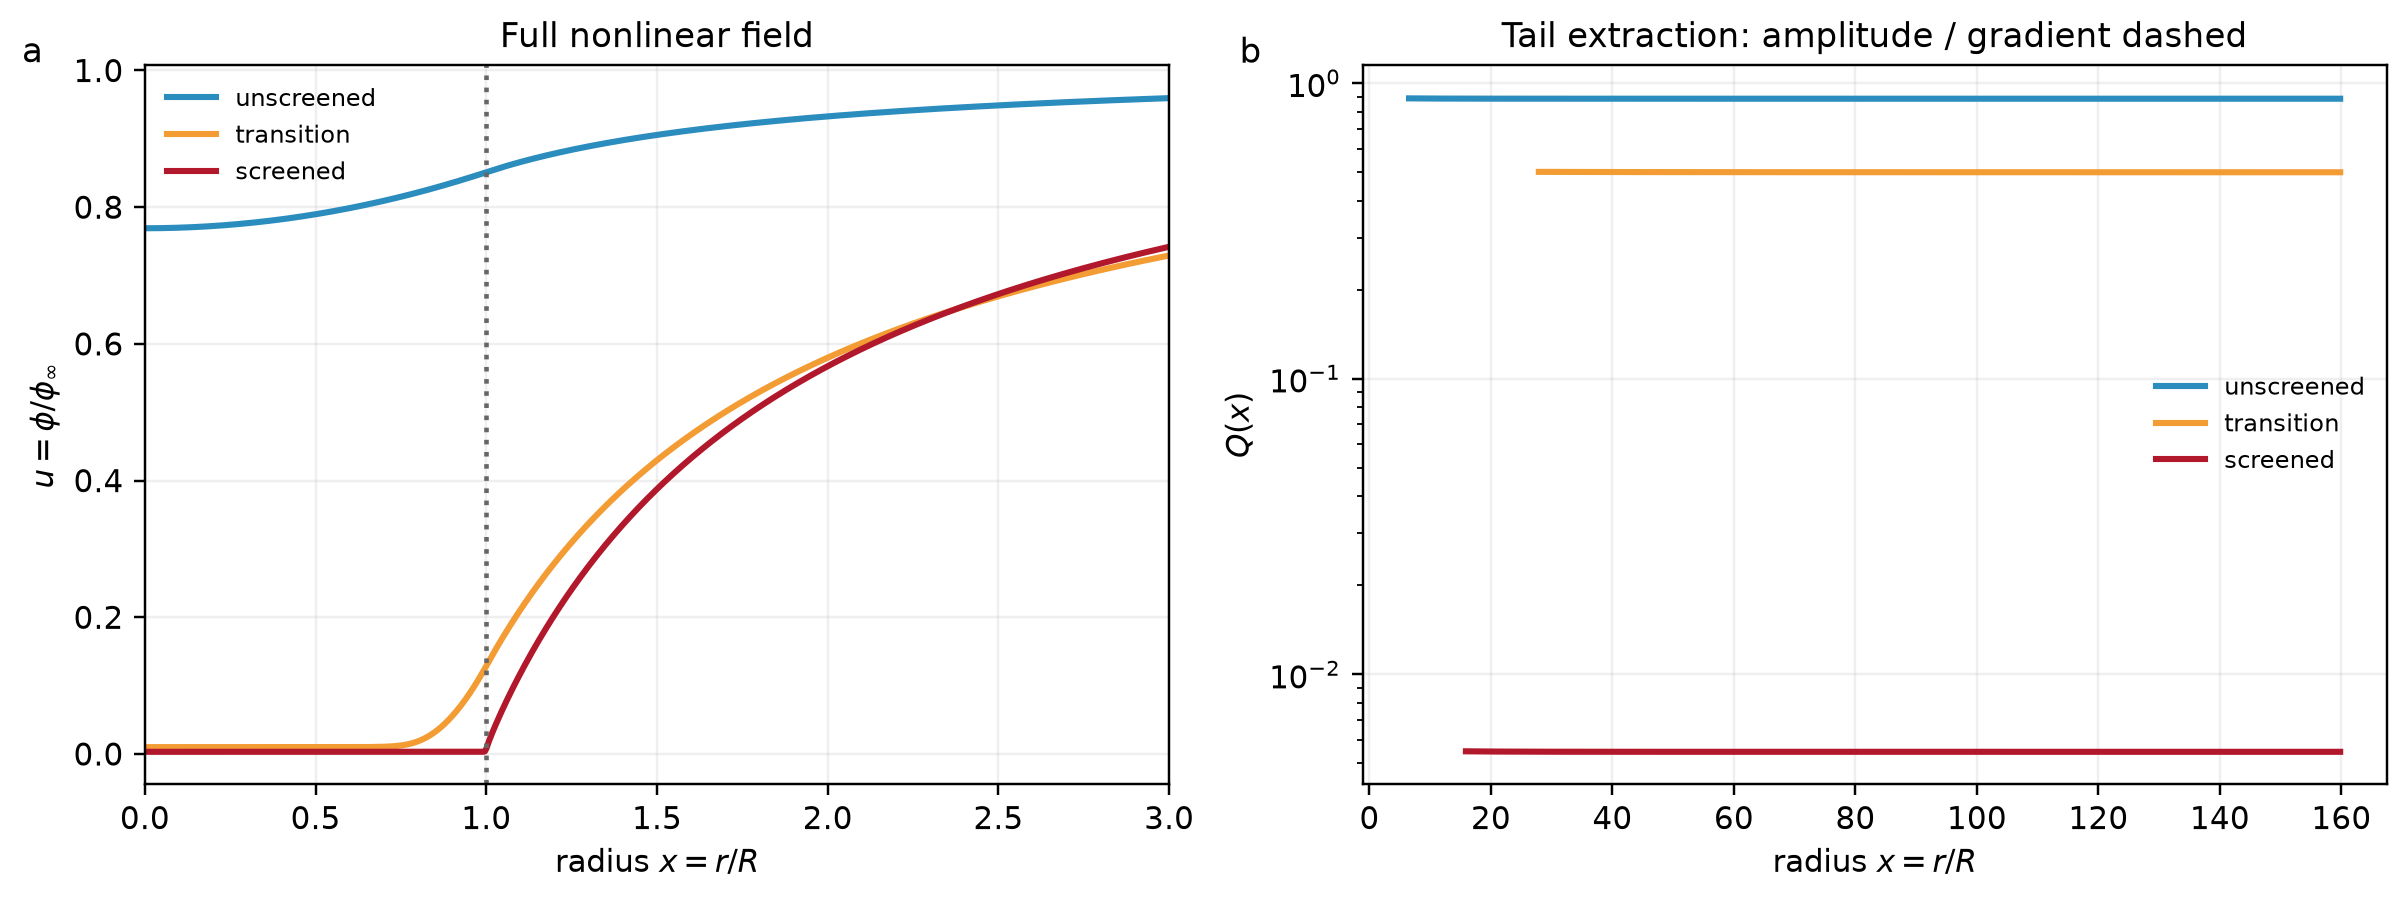
\includegraphics[width=.94\textwidth]{profiles_and_charge_extraction.png}
 \caption{비차폐, 전이, 강한 차폐의 대표 해. 외부 장의 점근 구간에서 전하 평탄부를 추출한다.}
\end{figure}
\begin{figure}[H]\centering
 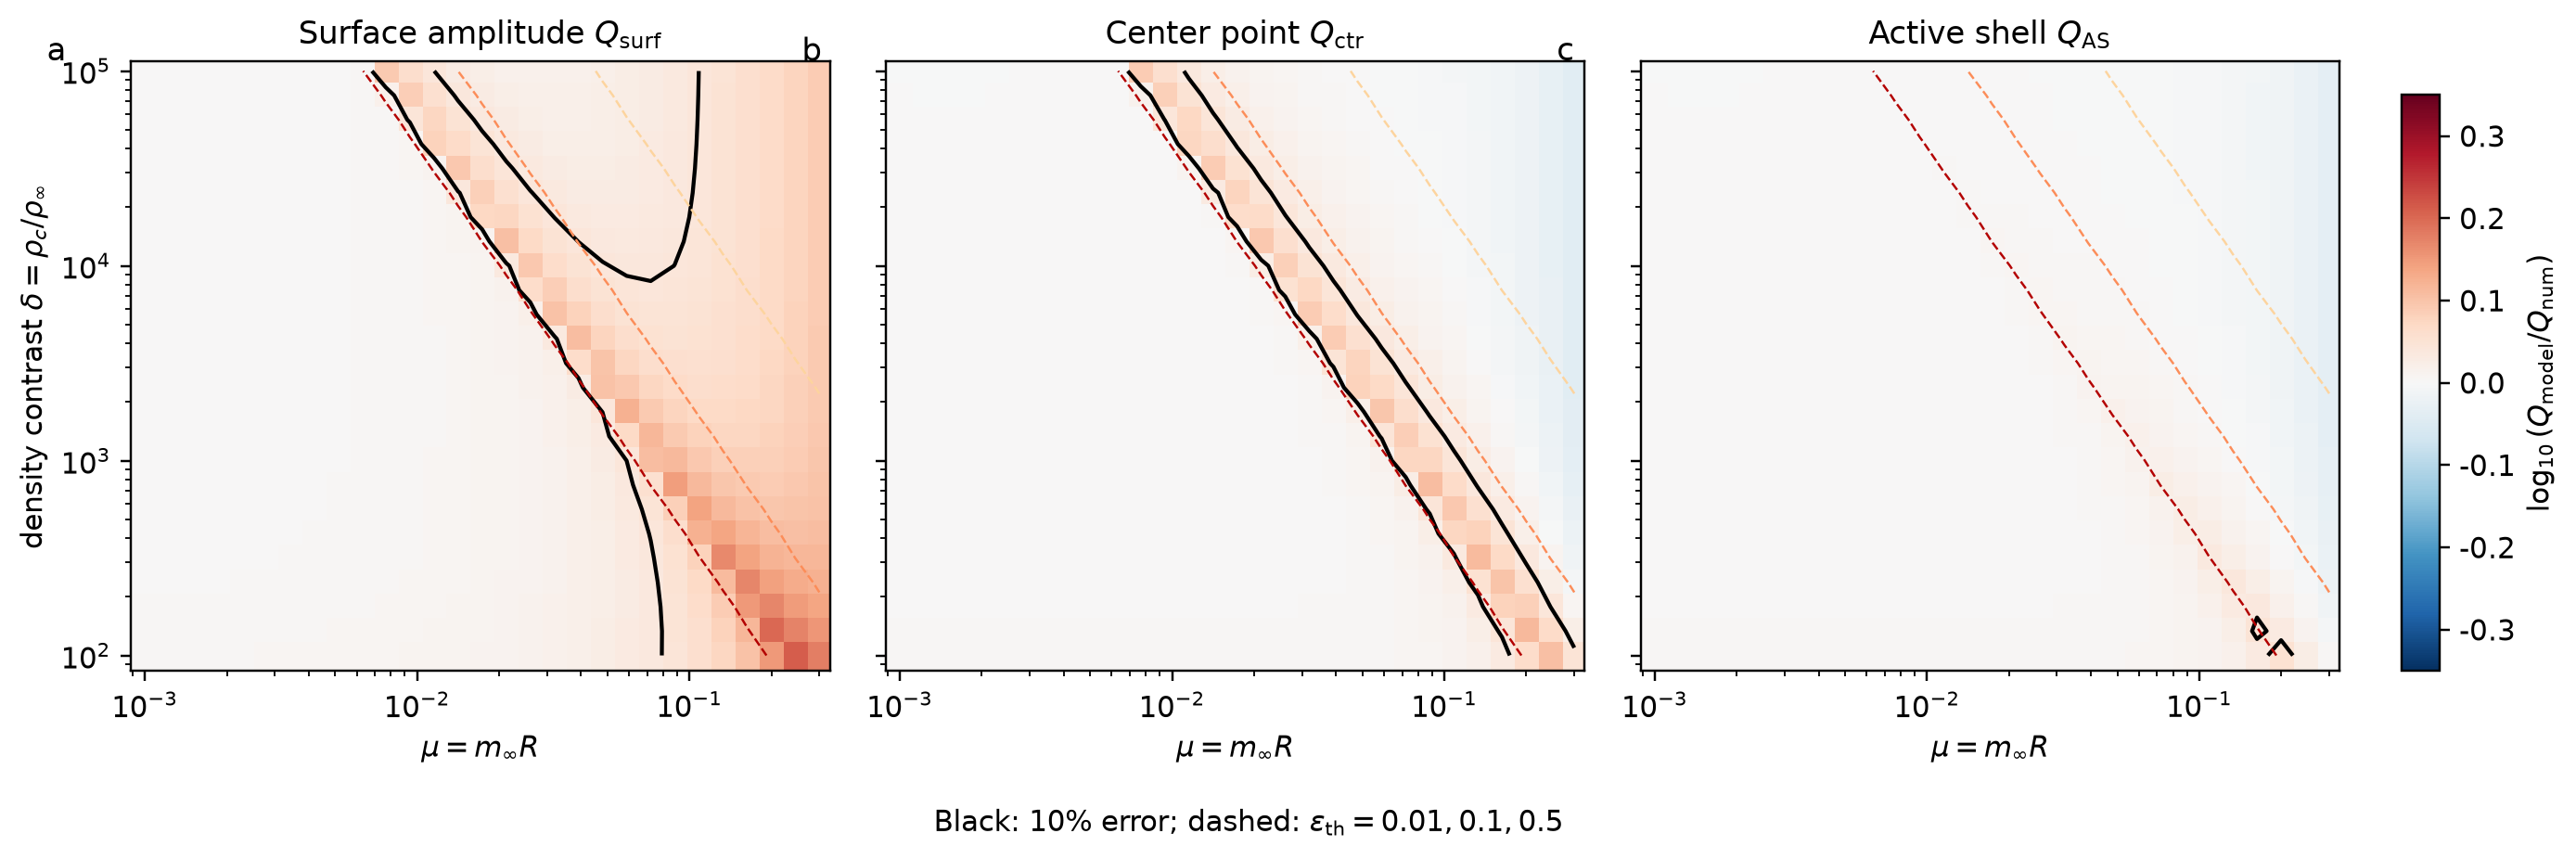
\includegraphics[width=\textwidth]{accuracy_atlas.png}
 \caption{수치적 점근 전하에 대한 부호 있는 전하 오차. 검은 곡선은 10\% 오차를
 나타낸다. 앞의 두 패널은 하나의 공통 정규화에서 서로 다른 유한 범위 진폭
 가설을 비교한다.}
\end{figure}
\begin{table}[H]\centering\small
 \caption{로그 격자에서의 전하 오차. 표본 중의 비율은 확률을 뜻하지 않는다.}
 \begin{tabular}{lrrr}\toprule
 모형 & 오차 중앙값 & 최대 오차 & 10\% 이내\\\midrule
 \StudyChargeRowsKO
 \bottomrule\end{tabular}
 \label{tab:charge}
\end{table}
간단한 $\qpv$와 방사형 적분은 모두 \StudyASWithin\%의 표본에서 10\% 목표를
달성한다. 전자는 오차 중앙값과 최댓값이 더 작고, 적분 모형은 데이터에 기록된
90백분위 오차가 조금 작다. 추가 반지름 가중치가 $\qpv$를 바꾸는 정도는 이
격자에서 최대 \StudyRadialMax\%이다. 결과는 유한 부피와 유카와 인자를 결합한
보정의 효과를 지지하지만, 관측된 성능 향상에 반지름 가중치가 필수적임을
입증하지는 않는다.

\begin{figure}[H]\centering
 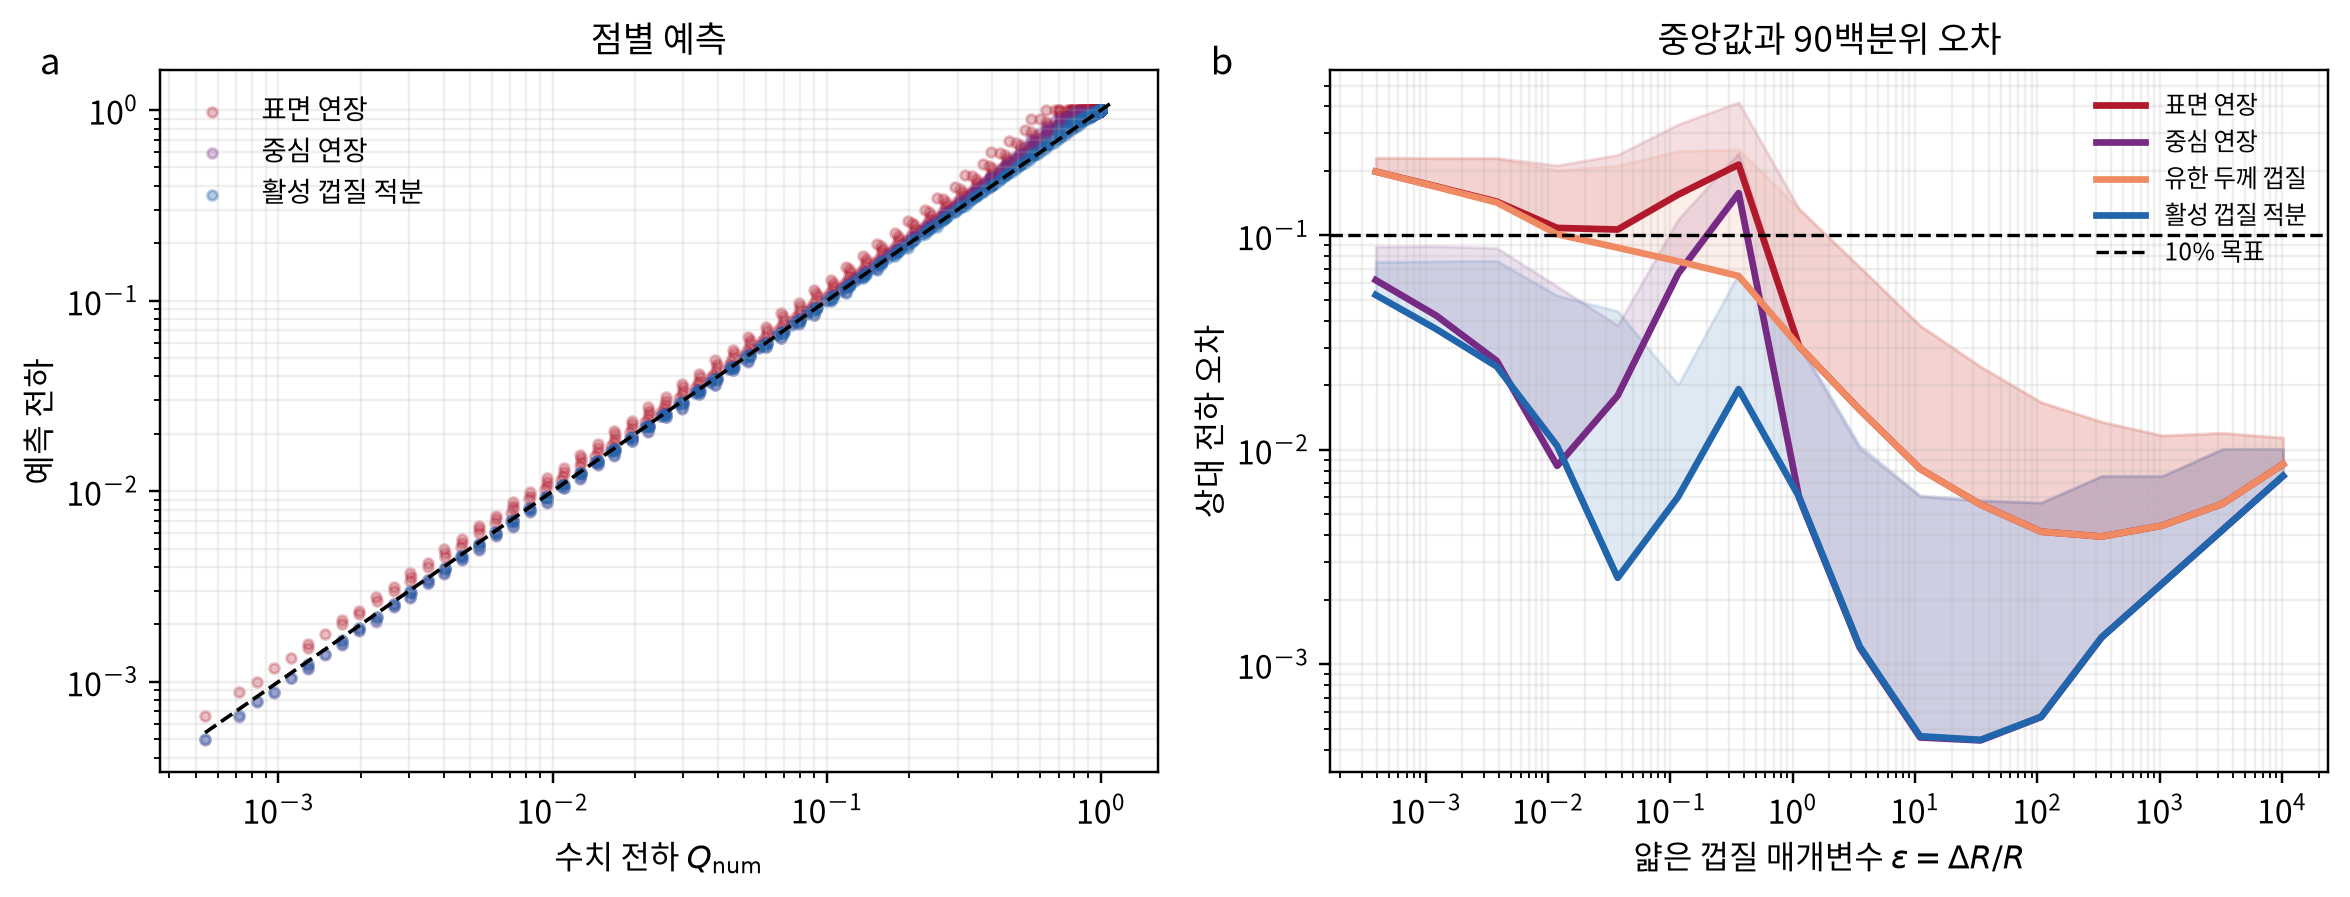
\includegraphics[width=\textwidth]{charge_comparison.png}
 \caption{대조군을 추가한 전하 비교. 회색 파선은 점원천 인자와 유한 부피를 결합한
 모형이다. 음영은 $\eps$ 구간별 중앙값부터 90백분위까지의 오차를 나타낸다.}
\end{figure}

경험적 장거리 전하 필터 $\eps<0.1$, $m_cR>10$, $\mu<0.035$는
\StudyGatePoints 개 격자점(전체의 \StudyGateCoverage\%)과 별도로 계산한
\StudyGateHeldout 개 로그 중점에서 10\% 목표를 통과한다. 이는 좁은 영역의 경험적
검사이며 보편적인 충분조건이 아니다. 이 고밀도 대비 격자에서는
$\eps(m_cR)^2=2(\sqrt\delta-1)$이므로 $\eps<0.1$이면 $m_cR>10$ 조건도
자동으로 만족한다. 이 주사만으로는 두 조건의 역할을 독립적으로 검증할 수 없다.

\subsection{점근 꼬리 힘의 거리별 유효성}
\begin{figure}[H]\centering
 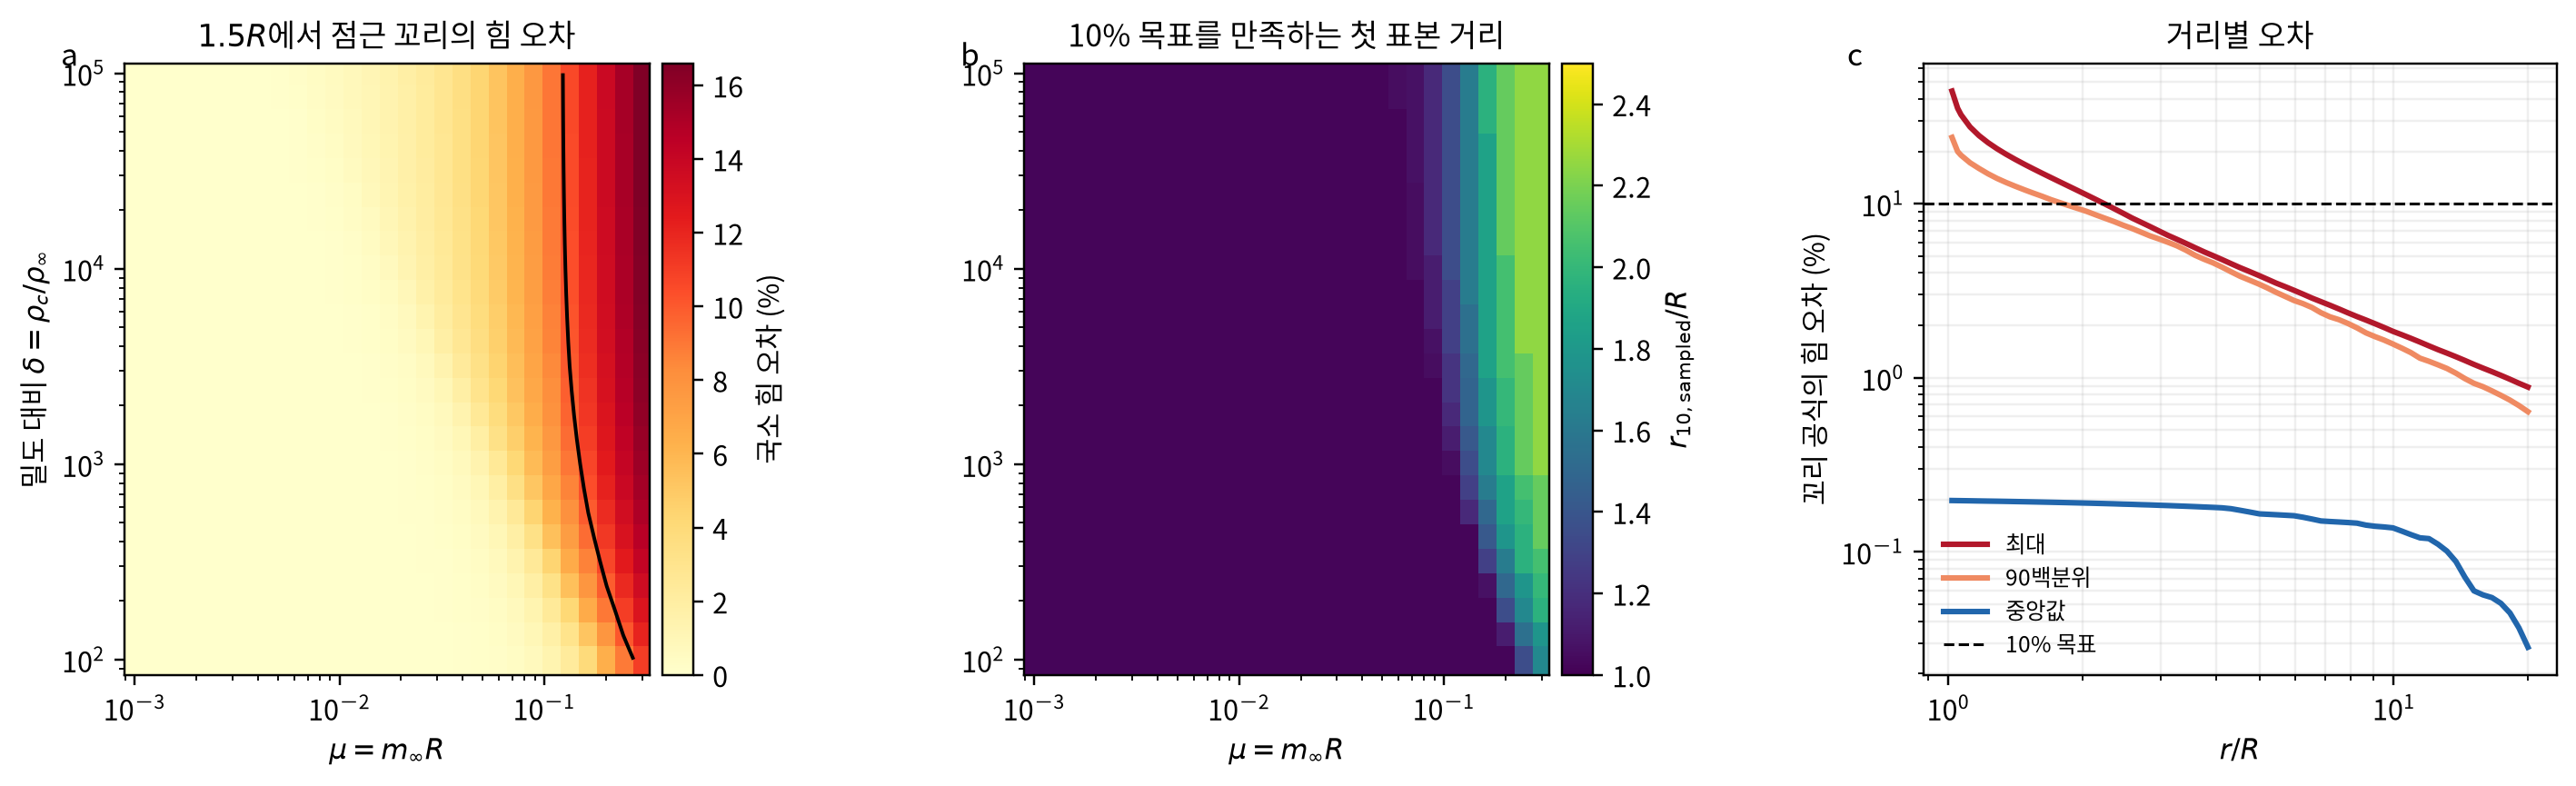
\includegraphics[width=\textwidth]{force_validity_map.png}
 \caption{(a) 수치 전하 자체를 사용했을 때 $1.5R$의 힘 오차. (b) $20R$까지 모든
 더 먼 표본에서도 10\% 목표를 유지하는 첫 표본 거리. (c) 거리별 오차 통계.
 표본 사이의 연속적인 유효성이나 $20R$ 바깥까지의 유효성을 증명한 경계는 아니다.}
 \label{fig:distance}
\end{figure}
\begin{table}[H]\centering\small
 \caption{수치적 점근 전하의 꼬리 공식과 직접 비선형 기울기의 힘 비교.}
 \begin{tabular}{rrrr}\toprule
 $r/R$ & 오차 중앙값 & 최대 오차 & 10\% 초과 표본\\\midrule
 \StudyDistanceRows
 \bottomrule\end{tabular}
\end{table}
점근 전하를 정확히 알아도 근거리 전파 오차는 남는다. $1.5R$에서는
\StudyForceNearFailures 개 점에서 오차가 10\%를 넘고, 최대 오차는
\StudyForceNearMax\%이다. 계산한 거리 표본에서는 $r/R=\StudyValidityRadiusMax$까지
모든 격자점이 10\% 목표에 도달하고, 그보다 먼 모든 표본에서도 목표를 유지한다.
고정된 $5R$, $10R$ 단면의 최대 오차는 각각 \StudyForceFiveMax\%,
\StudyForceTenMax\%로, 해당 표본 거리에서 더 작은 오차를 확인할 수 있다.

\begin{table}[H]\centering\small
 \caption{동일한 전하 근사식으로 $1.5R$의 국소 힘을 예측한 오차.}
 \begin{tabular}{lrrr}\toprule
 모형 & 오차 중앙값 & 최대 오차 & 10\% 이내\\\midrule
 \StudyLocalForceRowsKO
 \bottomrule\end{tabular}
\end{table}
예를 들어 $\qas$의 전하 목표 달성 비율은 \StudyASWithin\%이지만, 이 거리의
국소 힘에서는 \StudyASLocalWithin\%이며 최대 오차도 \StudyASLocalMax\%이다.
이는 식 \eqref{eq:factorization}의 오차 분해와 일치하며, 전하에 대한 좋은
벤치마크만으로 국소 힘의 정확도를 보장할 수 없음을 보여 준다.

\subsection{직접 힘을 기준으로 한 임계값 판정}
지도는 $1.5R$에서 식 \eqref{eq:direct}를 수치적 기준값으로 사용하고,
$\alpha_\star=\StudyThreshold$를 예시 임계값으로 택한다. $\qnum$을 넣은 꼬리
공식은 직접 힘과 \StudyTailFlips 개 점에서 판정이 다르다. 표면 진폭 가설과
중심점 가설은 직접 힘과 각각 \StudySurfaceFlips 개, \StudyCenterFlips 개 점에서
판정이 다르며, 등고선 이동의 중앙값은 각각 $\StudySurfaceShift$ dex와
$\StudyCenterShift$ dex이다. 이는 로그 격자 보간값이며 연속 경계를 정밀하게
해상한 결과는 아니다. 두 가설끼리 다른 판정을 내리는 점은
\StudyAnsatzDisagreement 개이고, 두 가설이 모두 직접 힘의 판정과 다른 점은
이 임계값에서 \StudyBothWrong 개이다.

\begin{figure}[H]\centering
 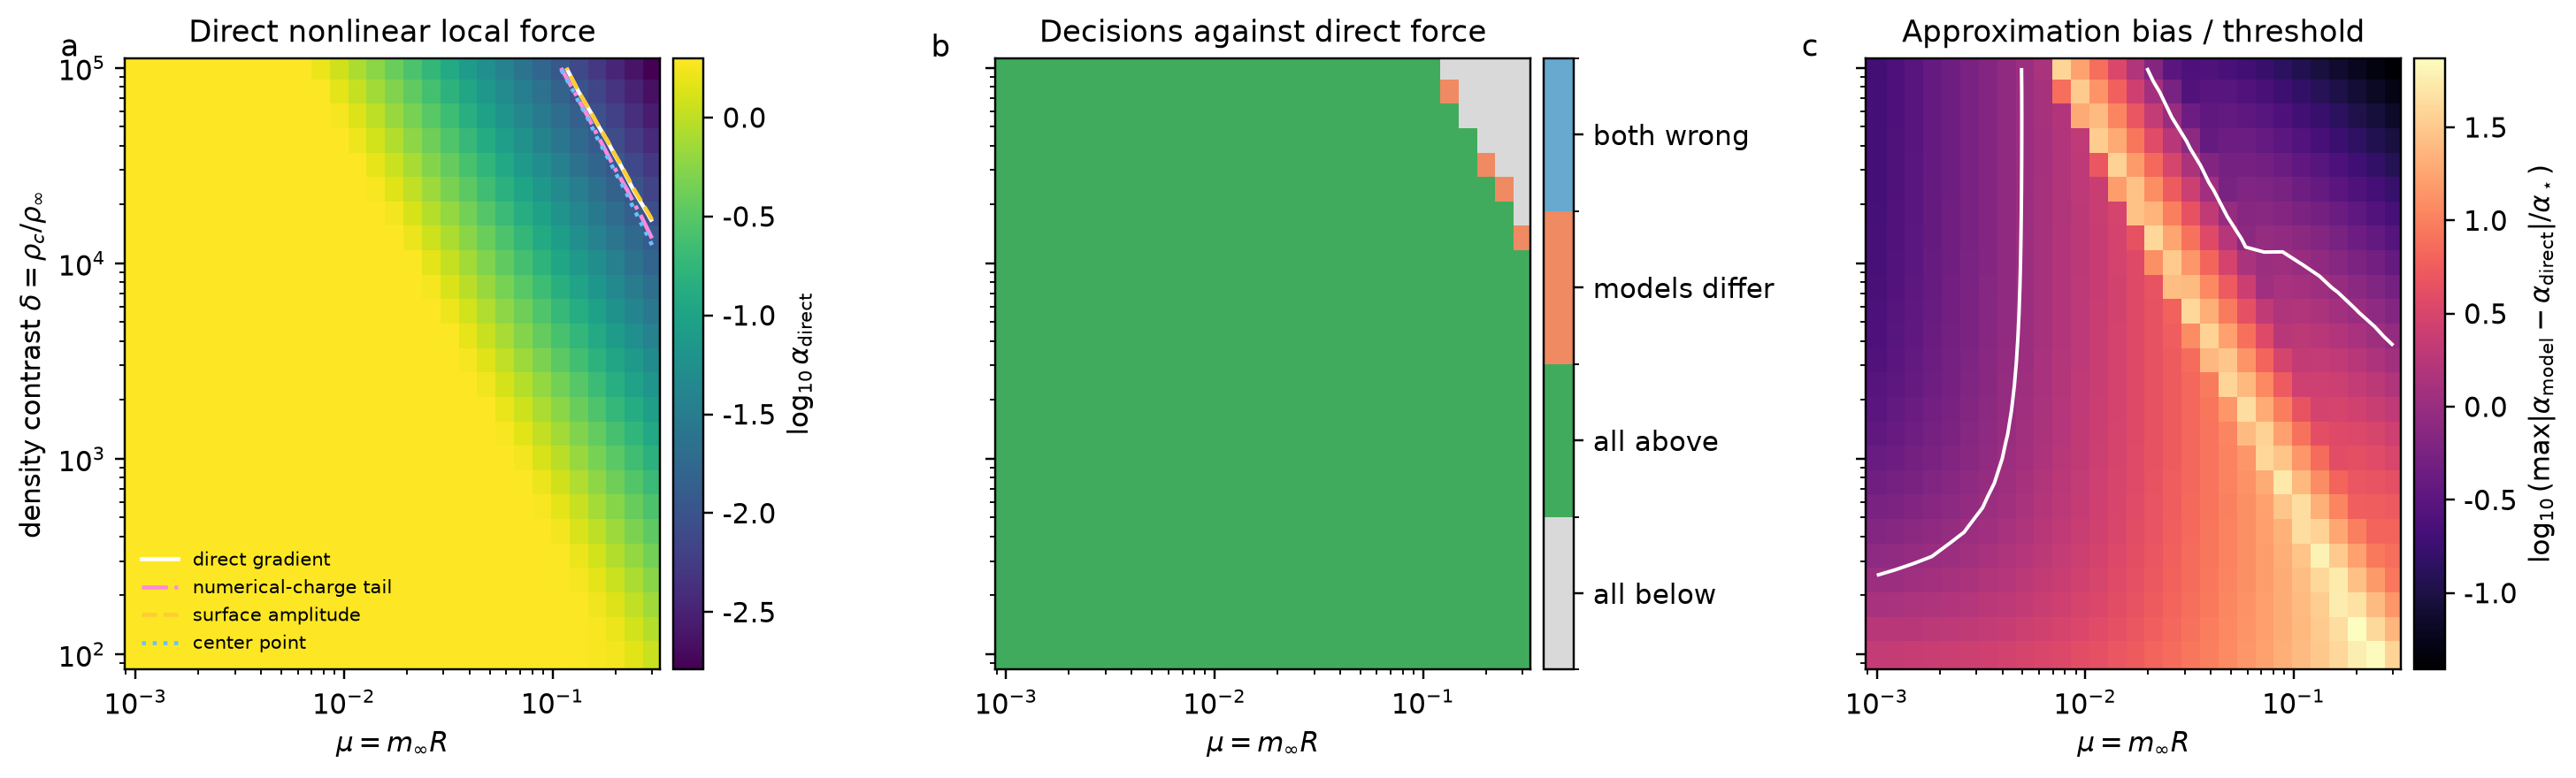
\includegraphics[width=\textwidth]{detectability_map.png}
 \caption{국소 힘비 임계값 지도. 흰 곡선은 직접 기울기의 임계선이다. 수치 전하의
 꼬리 공식과 두 단순 진폭 예측을 별도 곡선으로 표시한다. 세 번째 패널은 두
 단순 근사 중 큰 편향을 선택한 임계값으로 나눈 값이다.}
\end{figure}
별도의 민감도 표는 $\alpha_\star=0.001,0.003,0.01,0.03,0.1,0.3,1$을 다룬다.
모든 점이 임계값 위나 아래에 있는 경우도 정상적인 결과다. 격자를 지나는
임계선이 없으면 이동량을 null, 즉 해당 없음으로 기록한다. 하나의 임계값에서
얻은 판정 통계를 임의의 임계값으로 일반화하지 않는다.

\section{해석, 한계, 재현 방법}
뒷받침되는 연구 결과는 전하 오차와 유한 거리 가속도 오차의 구분, 그리고
직접 검증한 거리 의존성이다. 대조군은 이 제한된 격자의 전하 정확도 달성에
더 복잡한 방사형 적분이 필수적이지 않음도 보여 준다. $\mu\gtrsim1$, 다른
퍼텐셜과 원천 형상에서 이 관계가 달라지는지는 열린 문제이며, 추가 수치 검증과
기존 정합해에 대한 더 넓은 비교가 필요하다.

모형은 정적이고 구대칭이며, 각 영역의 밀도가 균일하고, 비상대론적이다.
$n=1$, $D\to0$에 조건부로 성립한다. 실제 실험에는 원천의 물리적 크기,
챔버 벽, 유한한 시험 물체의 반응, 원천 변조, 검출기 잡음과 계통 오차가 추가로
필요하다. 기존 원자 간섭계와 부유형 힘 센서 실험은 이러한 요소의 중요성을
보여 준다 \cite{Hamilton2015,Sabulsky2019,Yin2022}. 이 고립된 구 모형은 새로운
물리적 $(\Lambda,M_c)$ 배제 영역을 제시하거나 해당 실험들을 재평가하지 않는다.
실제 실험 예측에는 임의의 힘비 절단값 대신 예측한 차등 신호와 그 불확실성의
비를 사용해야 한다.

저장소 루트에서 다음을 실행한다.
\begin{verbatim}
python -m Thin_Shell_Study.run_study --workers 4 --force
python -m unittest discover -v
\end{verbatim}
첫 명령은 두 언어의 그림, 전하·국소 힘 CSV, 거리 및 임계값 민감도 표, 정밀
검증, JSON 지표, 두 보고서와 발표자료가 공유하는 수치 TeX 입력을 생성한다.
캐시에는 스키마와 수치 모형·설정의 해시를 저장하며, 전하만 있거나 코드·설정이
다른 캐시는 다시 계산한다. JSON에는 패키지 버전, 해시와 실행 시점의 Git
리비전도 기록한다. 한국어 그림만 다시 만드는 명령도 같은 지표와 임계값을
읽으며 독립적인 수치 기본값을 두지 않는다.

\section{결론}
수치적 전하 벤치마크는 재현되지만, 그것만으로 원천 가까이의 힘 벤치마크까지
성립하지는 않는다. 점원천 인자와 유한 부피를 결합한 대조군은 활성 껍질 적분과
같은 전하 목표 달성 비율을 보이므로, 반지름 가중치의 인과적 역할에 대한 주장을
제한해야 한다. 직접 기울기와 비교하면 점근 꼬리 힘의 최대 오차는 $1.5R$에서
\StudyForceNearMax\%이며, 이 격자의 $5R$와 $10R$에서는 각각
\StudyForceFiveMax\%, \StudyForceTenMax\%로 감소한다. 국소 힘을 기준으로
삼으면 선택한 임계값에서 \StudyTailFlips 개 판정이 바뀐다. 이는 차폐된 원천과
고전역학 관측량 사이에 사용하는 근사의 정확도를 구체적으로 검증하는 방법을 제공한다.

\clearpage
\begingroup\raggedright
\begin{thebibliography}{99}
\bibitem{KhouryPRL} J. Khoury and A. Weltman,
``Chameleon Fields: Awaiting Surprises for Tests of Gravity in Space,''
\emph{Phys. Rev. Lett.} \textbf{93}, 171104 (2004).
\href{https://doi.org/10.1103/PhysRevLett.93.171104}{doi:10.1103/PhysRevLett.93.171104}.
\bibitem{KhouryPRD} J. Khoury and A. Weltman, ``Chameleon Cosmology,''
\emph{Phys. Rev. D} \textbf{69}, 044026 (2004).
\href{https://doi.org/10.1103/PhysRevD.69.044026}{doi:10.1103/PhysRevD.69.044026}.
\bibitem{TamakiTsujikawa} T. Tamaki and S. Tsujikawa,
``Revisiting Chameleon Gravity: Thin-Shell and No-Shell Fields with Appropriate Boundary Conditions,''
\emph{Phys. Rev. D} \textbf{78}, 084028 (2008).
\href{https://doi.org/10.1103/PhysRevD.78.084028}{doi:10.1103/PhysRevD.78.084028}.
\bibitem{BurrageSakstein} C. Burrage and J. Sakstein, ``Tests of Chameleon Gravity,''
\emph{Living Rev. Relativ.} \textbf{21}, 1 (2018).
\href{https://doi.org/10.1007/s41114-018-0011-x}{doi:10.1007/s41114-018-0011-x}.
\bibitem{BurrageCopelandHinds} C. Burrage, E. J. Copeland, and E. A. Hinds,
``Probing Dark Energy with Atom Interferometry,'' \emph{JCAP} \textbf{03}, 042 (2015).
\href{https://doi.org/10.1088/1475-7516/2015/03/042}{doi:10.1088/1475-7516/2015/03/042}.
\bibitem{Hamilton2015} P. Hamilton et al., ``Atom-Interferometry Constraints on Dark Energy,''
\emph{Science} \textbf{349}, 849--851 (2015).
\href{https://doi.org/10.1126/science.aaa8883}{doi:10.1126/science.aaa8883}.
\bibitem{Elder2016} B. Elder et al., ``Chameleon Dark Energy and Atom Interferometry,''
\emph{Phys. Rev. D} \textbf{94}, 044051 (2016).
\href{https://doi.org/10.1103/PhysRevD.94.044051}{doi:10.1103/PhysRevD.94.044051}.
\bibitem{Schlogel2016} S. Schl\"ogel, S. Clesse, and A. F\"uzfa,
``Probing Modified Gravity with Atom Interferometry: A Numerical Approach,''
\emph{Phys. Rev. D} \textbf{93}, 104036 (2016).
\href{https://doi.org/10.1103/PhysRevD.93.104036}{doi:10.1103/PhysRevD.93.104036}.
\bibitem{Sabulsky2019} D. O. Sabulsky et al.,
``Experiment to Detect Dark Energy Forces Using Atom Interferometry,''
\emph{Phys. Rev. Lett.} \textbf{123}, 061102 (2019).
\href{https://doi.org/10.1103/PhysRevLett.123.061102}{doi:10.1103/PhysRevLett.123.061102}.
\bibitem{Yin2022} P. Yin et al.,
``Experiments with Levitated Force Sensor Challenge Theories of Dark Energy,''
\emph{Nature Phys.} \textbf{18}, 1181--1185 (2022).
\href{https://doi.org/10.1038/s41567-022-01706-9}{doi:10.1038/s41567-022-01706-9}.
\end{thebibliography}
\endgroup

\end{document}
